\documentclass{beamer}
\usepackage{HECbeamer}
% \usepackage{pgfpages}
% \pgfpagesuselayout{4 on 1}[letterpaper, landscape, border shrink=5mm]
\title[\color{white}{MATH 60604A\S~7e - Log rank test}]{\texorpdfstring{MATH 60604A\\Statistical modelling \\ \S~7e - Log rank test}{MATH 60604A\\ Statistical modelling \\ \S~7e - Log rank test}}
\author{}
\institute{HEC Montréal\\
Department of Decision Sciences}
\date{} 

\begin{document}
\frame{\titlepage}

 \begin{frame}
\frametitle{Comparing survival curves}
Recall the breast cancer trial data
\begin{itemize}
\vp \vp
\item \code{time}: time until death, or end of study in months
\item \code{death}: death indicator,  \code{0} for survivors, \code{1} for deceased
\item \code{im}: response to immunohistochemical examination, either negative (\code{0}) or positive (\code{1})
\end{itemize}
Suppose we're interested in seeing whether survival function is different for those who respond positively relative to those who respond negatively to the immunohistochemical examination.
\begin{itemize}
\vp \vp
\item Do women who respond positive to the immunohistochemical examination tend to survive longer than those who respond negatively?
\end{itemize}

\end{frame}

\begin{frame}[fragile]
\frametitle{Compararison of survival curves}
We specify the group variable through the command \code{strata}.
\vp \vp
\begin{tcolorbox}[colback=white,colframe=hecblue,title=\SASlang{}]
{ \footnotesize 
\begin{verbatim}
proc lifetest data=statmod.breastcancer method=km plots=(s);
time time*death(0);
strata im;
run;
\end{verbatim}
}
\end{tcolorbox}
{\footnotesize 

\SASlang{} will estimate the survival curve separately for individuals in the two \code{im} groups.


}
\end{frame}
\begin{frame}[fragile]
\frametitle{Survival curves (Kaplan--Meier)}
\begin{center}
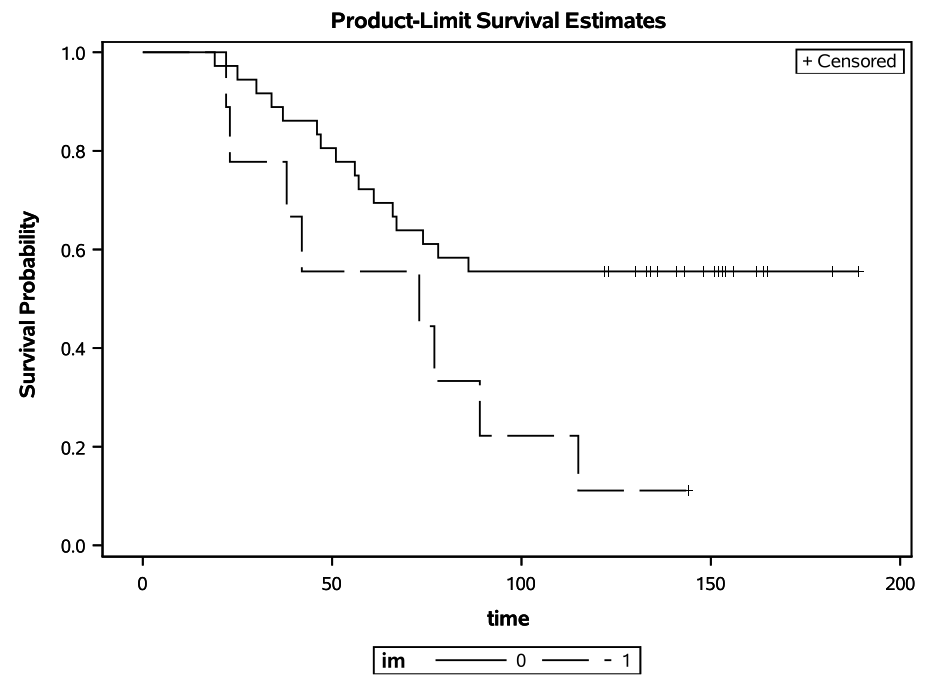
\includegraphics[width = 0.7\textwidth]{img/c7/slides7e15}
 \end{center}
\end{frame}

\begin{frame}
\frametitle{Comparison of survival curves}
It seems that women with a negative immunohistochemical examination response (\code{im=0}) have \alert{better} survival than those who have a positive response (\code{im=1}).
\begin{itemize}
\item For most times $t$, $\widehat{S}_1(t) > \widehat{S}_2(t)$ so that those with \code{im=0} have higher survival probability than those with \code{im=1}.
\end{itemize}
But is is the survival function significantly different in the two groups \code{im=0} and \code{im=1}?
\begin{itemize}
\vp \vp
\item[] $\Hy_0: S_1(t) = S_2(t)$ for all $t$,
\item[] $\Hy_1: S_0(t) \neq S_1(t)$ for at least one value of $t$.
\end{itemize}
\end{frame}

\begin{frame}[fragile]
\frametitle{Log rank test}
 Consider Cox's proportional hazard regression model of the form
 \begin{align} 
  h(t) = h_0(t)\exp(\beta \code{im}). \tag{$\star$} \label{lograngtest}
 \end{align}
\bi 
\item The null hypothesis of equality of survival functions amounts to testing $\Hy_0: \beta=0$. 
\item The score statistic can be used to test this hypothesis without fitting the model 
\bi 
\item under $\Hy_0$, the estimated hazard yields Kaplan--Meier's estimator.
\ei
\item The score test requires calculating the gradient and the hessian of the model \eqref{lograngtest} and evaluating them at $\beta=0$ 
\bi 
\item both are simple function of the number of individuals at risk each time $t_i$. 
\ei
 \ei
\end{frame}
% \begin{frame}
%  \frametitle{Log rank statistic}
% 
%  
%  For two groups with no ties, we get
%  \begin{align*}
% \left.U(\beta)\right|_{\beta=0}& = \sum_{i: \delta_i=1} \left(g_i - \frac{r_{i1}}{r_{i0}+r_{i1}}\right), 
% \\\left.j(\beta)\right|_{\beta=0}&= \sur_{i: \delta_i=1} \frac{r_{i0}r_{i1}}{(r_{i0} + r_{i1})^2}
%  \end{align*}
% where 
% \bi \item $g_{i}=1$ is individual experiencing the event at time $t_i$ belongs to groupe 1 and $g_i=0$ otherwise.
% \item $r_{ij}$ is the number of individuals at risk at time  $t_i$ in group $j$.
% \ei
% \end{frame}
\begin{frame}[fragile]
\frametitle{Proportional hazard model}
\begin{tcolorbox}[colback=white,colframe=hecblue, title=\SASlang{} code to fit a proportional hazard model]
\begin{verbatim}
proc phreg data=statmod.breastcancer;
model time*death(0) = im / ties=exact;
run;
\end{verbatim}
\end{tcolorbox}
\begin{center}
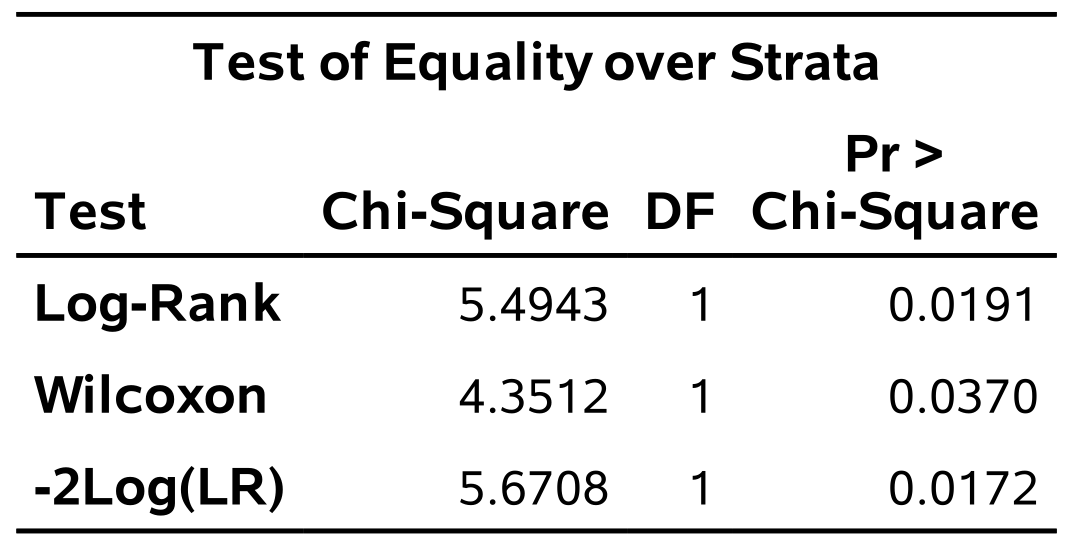
\includegraphics[width = 0.45\textwidth]{img/c7/slides7e16}
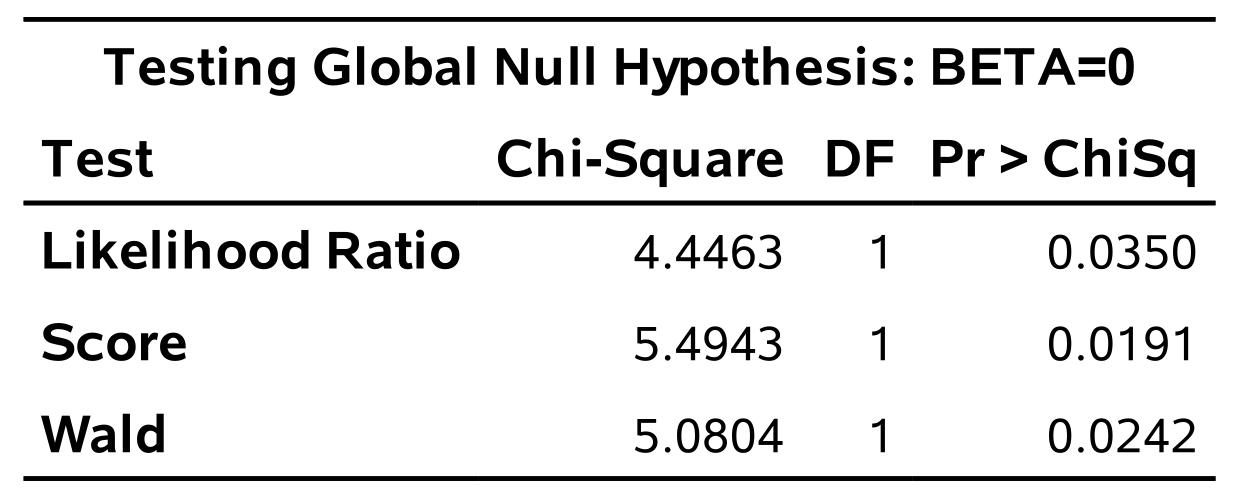
\includegraphics[width = 0.51\textwidth]{img/c7/slides7e17}
\end{center}
{\footnotesize 

The log rank test is also displayed by default in the \SASlang{} output of the \code{lifetest} procedure (left).

}
\end{frame}

\begin{frame}
\frametitle{Log rank test}
\bi 
\item Under $\Hy_0: \beta=0$, the null distribution of the score statistic is approximately $\chi^2_1$.
\item The $p$-value is $0.0191$: we reject $\Hy_0$ at level $5\%$ and conclude that the survival curves are different for women with negative / positive responses to the immunohistochemical examination.
\item We can generalize the log rank test by using a Cox model with a $k$ level categorical variable as sole predictor: 
\bi \item the null distribution of the test statistic is then $\chi^2_{k-1}$.
\ei
\ei 
\end{frame}

\end{document}
